\section{Activation Record(活动记录)}
\subsection{Stack Frame(栈帧)}
活动记录就是栈帧. 

\begin{definition}
    栈中存放函数的局部变量/参数/返回地址/临时变量的这片区域为该函数的活动记录 (activation record) 或栈帧(stack frame).
\end{definition}
\begin{figure}[H]
    \centering
    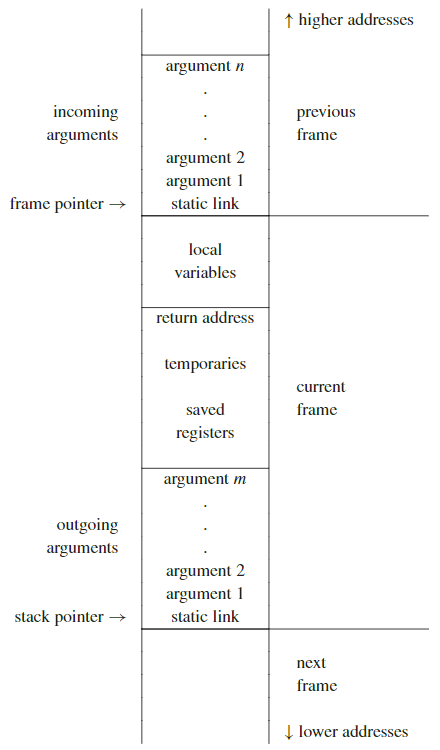
\includegraphics[width=0.6\linewidth]{pic/CP678/a typical stack frame layout.png}
    \caption{a typical stack frame layout}
\end{figure}
\begin{itemize}
    \item incoming arguments: 是前一个帧的一部分, 但其与 frame pointer 的偏移量已知.
    \item return address: 由 CALL 指令创建, 告知完成此函数后需要返回何处.
    \item local variables: 一些在帧中, 一些在寄存器上. 在寄存器与帧中临时空间之间移动.
\end{itemize}

\subsection{Frame Pointer}
\begin{itemize}
    \item Frame Pointer/Base Pointer: 基址寄存器
    \item Stack Pointer: 栈顶寄存器
\end{itemize}

帧指针的变化:一个函数 $f$ 调用 $g(a_1,a_2,\dots)$ 时,
进入g:
\begin{enumerate}[start=1]
    \item sp 指向第一个参数 $a_1$
    \item 将旧的fp压入栈
    \item 令新的fp=sp
    \item sp 减去栈帧大小(向低地址增长)得到新的 sp
    \item $g$ 可以基于 fp 向高地址获取参数, 或基于 sp 向低地址压入/查询局部变量
\end{enumerate}
从g退出: 
\begin{enumerate}[start=6]
    \item 返回值拷贝至特殊寄存器
    \item sp=fp (释放 $g$ 的栈帧)
    \item 从栈上取回旧的 fp 值到 fp 中
\end{enumerate}

\subsection{Parameter Passing}
调用函数需要保护现场: 因为寄存器的值可能会被子函数改变, 返回时``现场已经被破坏''. 为此部分寄存器的值需要在栈上进行备份. 分为以下两种: 
\begin{itemize}
    \item Caller-save: 例如临时寄存器, 调用者如果用到则需要自己保存, 子函数可以任意修改.
    \item Callee-save: 例如fp/sp, 由子函数负责保存与恢复(进入子函数时push到栈, 退出时从栈里pop), 调用者无需关心.
\end{itemize}


函数调用传参: 大部分现代编译器对于前几个参数直接通过寄存器传递, 多余的则仍然通过栈完成传递.

优化策略:
\begin{itemize}
    \item 从变量生命周期入手: 如果寄存器对应的变量或参数在当前函数不再使用, 子函数覆盖了自然也无妨.
    \item 全局寄存器分配策略: 每个函数使用不同的一组寄存器传参.
    \item 优化叶过程(Leaf Procedure): 如果某函数不调用任何其他过程, 自然也不需要为(不存在的)子过程备份传入的参数.
    \item 寄存器窗口Register Windows: 每次调用函数时, 尽可能利用尚未用到的寄存器, 然后为子函数分配新的一套可用的寄存器(SPARC采用该策略).
\end{itemize}

\subsection{Frame-Resident Variables}
寄存器并非万能: 有时, 在栈上分配空间(实体化)是不可避免的. 例如:
\begin{itemize}
    \item 对象过大, 无法放在寄存器中
    \item 数组对象, 需要通过地址偏移访问
    \item 寄存器被特殊需要, 例如上文提到可能用于传参
    \item 太多中间值/局部变量, 有限的寄存器放不下. 称为 Spill, 在寄存器分配部分会展开讨论
    \item 变量 逃逸(escape)(也就是脱离了当前scope/无法确定变量有效的生命周期): 
    \subitem 引用传参: 需要内存地址
    \subitem 显式地取变量地址
    \subitem 被嵌套函数访问
\end{itemize}

\subsection{Block Structure}
在允许函数嵌套定义的语言(比如Tiger)中, 内部函数可能使用外部函数中的局部变量. 为了使得内部函数访问非局部定义的外部变量, 有以下几种方法: 

静态链接: 当内部函数 $g$ 被调用时, 调用者 $f$ 传入一个指针指向 $f$ 的栈帧(或者说活动记录), 这种情况下, 称为 $f$ statically encloses $g$.  如果多次嵌套, 嵌套次数为$N$, 这些指针会构成一个长为 $N$ 的单向链表串联起栈帧. 每个函数记录自己的嵌套深度 $n$. 如果访问了在深度 $m$ 的变量, 只需沿着该链向上 $n-m$ 次就可以找到该变量所在的栈帧. 优缺点: Overhead小, 但是因为要通过链表向上经过多层速度较慢. 


Lamda lifting: 从最深的一层叶过程开始, 把所有 $g(a_1)$ 用到的外部变量 $o_1, o_2$ 改写为真正传入的参数, 于是变为$g(o_1, o_2, a_1)$. 如此逐渐向上改写每一层即可. 


Display数组: 一个全局数组, 记录当前每个嵌套深度 $i$ 对应的栈帧地址. 这样不需要经过链表即可直接找到变量对应的栈帧. 


\section{Translation to Intermediate Code}
intermediate represent(中 间 表 示): 抽象的机器语言,链接前端和后端,解决了高级语言和目标机器汇编语言之间的转化.

\begin{itemize}
    \item 前端(front end):词法分析,语法分析,语义分析,翻译成中间代码
    \item 后端(back end):IR 优化, 翻译成机器语言.
\end{itemize}

\subsection{Intermediate Representation Trees}
\subsubsection{Tree Operator}
Expressions(T\_exps): 
\begin{itemize}
    \item CONST($i$): 整 型 常 数 
    \item NAME($n$): 符 号 常 数 
    \item TEMP($t$): 临 时 变 量 
    \item BINOP($o, e_1, e_2$):对操作数 $e_1,e_2$ 的 二 元 操 作 
    \item MEM($e$):作为 MOVE 操作的左子式时表示对储存器 $e$ 地址的存入;其他位置表示读取该地址的内容 
    \item CALL($f,l$):过程调用 
    \item ESEQ($s,e$): 先计算语句 s 形成副作用,然后计算 $e$ 违该表达式的值 
\end{itemize}

Statements(T\_stm):
\begin{itemize}
    \item MOVE(TEMP $t, e$): 计算 $e$ 的值然后存到临时变量 $t$ 中
    \item MOVE(MEM($e_1$),$e_2$):计算 $e_2$ 的值然后存入到 $e_1$ 作为地址的内存中 
    \item JUMP($e$,$labs$):跳转到 $e$ 地址 或 者 $labs$ 为 label 的 地 址
    \item CJUMP($o,e_1,e_2,t,f$): 依 次 计 算 $e_1$ 和 $e_2$, 生成值 $a,b$;然后用比较运算符操作 $aob$,如果结果为 true 跳到 $t$,反之跳转到 $f$; 
    \item SEQ($s_1,s_2$):语句 $s_1$ 后 面 跟 $s_2$
    \item LABEL($n$):定会一名字后的常数值为当前机器代码的地址.
\end{itemize}


\subsection{Translation into Trees}
\subsubsection{Kinds of Expressions}
\begin{itemize}
    \item Ex 代表 expression
    \item Nx 代表无结果的 statement
    \item Cx 代表条件分支, 可能跳转到 true label 或 false label.
\end{itemize}

对于 CJUMP 和 JUMP 语句,还 不知道 label 的具体值,需要 使用两张表: 
\begin{itemize}
    \item 真值标号回填表 (true patch list)
    \item 假值标号回填表 (false patch list)
\end{itemize}

\subsubsection{Variables}
\begin{itemize}
    \item Simple variables: 
    \subitem MEM(BINOP(PLUS, TEMP $fp$, CONST $k$))
    \item Following static links:
    \subitem MEM(+(CONST $k_n$, MEM(+(CONST $k_{n-1}$, $\dots$ MEM(+(CONST $k_1$, TEMP $fp$))$\dots$))))
    \item Array variables: 
    \subitem MEM(+(MEM($e$), BINOP(MUL, $I$, CONST $W$)))
\end{itemize}

\subsubsection{Conditionals}
e.g. if $x<5$ then $a>b$ else 0, \\
$x<5$ translates into Cx($s_1$), $a>b$ translates into Cx($s_2$)

SEQ($s_1$($z$,$f$), SEQ(LABEL $z$, $s_2$($t$,$f$)))

\subsubsection{Loops}
\begin{itemize}
    \item while
    \begin{minted}{text}
    test:
        if not(condition) goto done
        body
        goto test
    done:
    \end{minted}
    
    \item for
    \begin{minted}{text}
    for i:=lo to hi         let var i:=lo
        do body                 var limit:=hi
                            in while i<=limit
                                do(body; i:=i+1)
                            end
    \end{minted}
    
\end{itemize}

\subsubsection{Function Call}
CALL(NAME $l_f$, [$sl, e_1, e_2,\dots, e_n$])

$l_f$ is the label for $f$, $sl$ is the static link

\subsection{Declarations}
变量声明将会在 frame 中额外保留部分空间;函数声明会在 Tree code 中保留一个新的 fragment.

变量的初值会被转换成一个 Tree 表达式,transDec 返
回一个 Tr\_Exp,这个 Tr\_Exp 应当包含完成赋初值的
赋值表达式;如果对函数和类型声明施加 transDec,
结果将会得到 Ex(CONST(0))这样的空操作

函数被翻译为入口代码 (prologue), 函数体 (body) 和出口函数 (epilogue) 组成的汇编语言代码.

入口包含:
\begin{enumerate}
    \item 声明一个函数开始的伪指令 (pseudo instructions)
    \item 函数名 label 的定义
    \item 调整栈指针的一条指令,用于分配新的栈帧
    \item 将逃逸(escaping)参数保存至栈帧的指令,以及将非逃逸参数传送的新临时寄存器指令
    \item 保 存  此 函 数 用 到 的 callee-save 寄存器(包括返回地址寄存器)
\end{enumerate}

本体:
\begin{enumerate}[start=6]
    \item 函数体
\end{enumerate}

出口包含:
\begin{enumerate}[start=7]
    \item 将返回值传送至专用于返回结果的寄存器 
    \item 用 于 恢 复 callee-save 的寄存器取数指令
    \item 恢 复 栈 指 针 , 释 放 栈 帧
    \item return 指令
    \item 声明函数结束的伪指令
\end{enumerate}


\section{Basic Blocks and Traces}

\subsection{Canonical Trees(规范树)}
\subsubsection{Definition}
\begin{definition}
    A canonical trees have these properties:
    \begin{enumerate}
        \item No SEQ or ESEQ
        \item The parent of each CALL is either EXP($\dots$) or MOVE(TEMP $t$, $\dots$).
    \end{enumerate}
\end{definition}

Why?
\begin{enumerate}
    \item CJUMP 能够跳转到两个标号的任意一个,但实际的是条件为假时跳转到下一条
    \item ESEQ 会使得子树的不同计算顺序产生不同结果
    \item 表达式使用 CALL 会有计算顺序不同的问题
    \item CALL 的嵌套调用(作为另一个 CALL 的参数)会出问题,覆盖存放返回值的寄存器的值
\end{enumerate}

重写流程:
\begin{enumerate}
    \item 一棵树重写成规范树 
    \item 将树分组合成不含转移和标号的基本块 (basic block) 集合 
    \item 对基本块 进行 排 序 形 成 一 组 轨 迹(trace);每一个 CJUMP 后就是其 false 标号
\end{enumerate}

\subsubsection{Transformations on ESEQ}
% \begin{enumerate}
%     \item ESEQ($s_1$, ESEQ($s_2$,$e$)) $\to$ ESEQ(SEQ( $s_1,s_2$), $e$) 
%     \item BINOP($op$,ESEQ($s$,$e_1$), $e_2$) \\
%     $\to$ ESEQ(BINOP($op$,$e_1$, $e_2$)) 
%     \subitem MEM(ESEQ($s$,$e_1$)) $\to$ ESEQ( $s$, MEM($e_1$)) 
%     \subitem JUMP(ESEQ($s$, $e_1$)) $\to$ SEQ($s$,JUMP($e_1$)) 
%     \subitem CJUMP(op,ESEQ($s$,$e_1$),$e_2$,$l_1,l_2$)\\
%     $\to$ SEQ($s$, CJUMP($op$, $e_1$, $e_2$, $l_1,l_2$)) 
%     \item BINOP(op,$e_1$, ESEQ(s,$e_2$))
%     $\to$ ESEQ(MOVE (TEMP t, $e_1$), ESEQ(s, BINOP(op, TEMP t, $e_2$))) 
%     \subitem CJUMP(op, $e_1$, ESEQ(s, $e_2$), $l_1,l_2$) $\to$ \\
%      SEQ(MOVE(TEMP $t$, $e_1$), SEQ($s$, CJUMP($op$, TEMP $t$, $e_2$, $l_1,l_2$))).
%      \item 如果 ESEQ 中 $s$ 和 $e_1$ 是 可 交 换 的 (commute), 那 么 可 以 直 接 把 $s$ 和 $e_1$ 交换,ESEQ 提出来
% \end{enumerate}

\begin{table}[H]
    \centering
    \small
    \caption{Transformations on ESEQ}
    \begin{tabular}[c]{L{0.44\linewidth}L{0.44\linewidth}}\toprule 
        Expression & Transforms to \\ \midrule
        ESEQ($s_1$, ESEQ($s_2$, $e$)) & ESEQ(SEQ( $s_1,s_2$), $e$) \\
        BINOP($op$, ESEQ($s$, $e_1$), $e_2$) & ESEQ(BINOP($op$,$e_1$, $e_2$)) \\
        MEM(ESEQ($s$, $e_1$)) & ESEQ($s$, MEM($e_1$))  \\
        JUMP(ESEQ($s$, $e_1$)) & SEQ($s$, JUMP($e_1$)) \\
        CJUMP(op, ESEQ($s$, $e_1$), $e_2$, $l_1,l_2$) & SEQ($s$, CJUMP($op$, $e_1$, $e_2$, $l_1,l_2$)) \\
        BINOP(op, $e_1$, ESEQ(s, $e_2$)) & ESEQ(MOVE (TEMP t, $e_1$), ESEQ(s, BINOP(op, TEMP t, $e_2$))) \\ 
        CJUMP(op, $e_1$, ESEQ(s, $e_2$), $l_1,l_2$) &  SEQ(MOVE(TEMP $t$, $e_1$), SEQ($s$, CJUMP($op$, TEMP $t$, $e_2$, $l_1,l_2$))). \\
        \bottomrule
    \end{tabular}
\end{table}
如果 ESEQ 中 $s$ 和 $e_1$ 是 可 交 换 的 (commute), 那 么 可 以 直 接 把 $s$ 和 $e_1$ 交换,ESEQ 提出来. 

\subsubsection{Moving CALLs to top level}
以 BINOP(op,CALL(),CALL() $\dots$) 为例, 第二个 CALL 会在 BINOP 执行前覆盖第一个CALL 返回在 RV 寄存器里的值. 解决办法是使用 ESEQ 将返回值保存到一个新的临时变 量里: CALL(fun,args) $\to$ ESEQ(MOVE(TEMP $t$, CALL(fun, args)), TEMP $t$)


\subsection{Taming Conditional Branches}
\subsubsection{Basic Blocks(基本块)}
取 一 列 规 范 树 , 块 的 开 始 是 label, 以跳转指令为结尾. 即:
\begin{enumerate}
    \item 第一个语句是 LABEL
    \item 最 后 一 个 语 句 是 JUMP 或 CJUMP
    \item 没 有 其 他 的 LABEL,JUMP 或 CJUMP
\end{enumerate}

划分基本块方法: 从头到尾扫描语句序列,每次发现一个 LABEL 就开始一个新的基本块并结束上一个基本块; 每发现一个 JUMP 或 CJUMP 就结束一个基本块(并开始下一个基本块). 如果过程还遗留任何基本块不是 JUMP 或 CJUMP 结尾的, 则在基本块块末尾增加一条转移到下一个基本快标号处的 JUMP; 如果有任何基本块不是以 LABEL 开始的, 则生成一个新的标号插入到基 本 块 开 始; 在全部 末 尾 添 加 done LABEL, 将 JUMP(NAME done) 放到最后一个基本快末尾.


\subsubsection{Trace(轨迹)}
程 序 执 行期间可能连贯执行的语句序列. 要寻找一组能够覆盖整个程序的轨迹集合, 且每一个基本块仅出现在一条轨迹中.
\begin{algorithm}[H]
    \caption{Generation of traces}
    \begin{algorithmic}
        \State Put all the blocks of the program into a list $Q$
        \While{$Q$ is not empty}
            \State Start a new (empty) trace, call it $T$.
            \State Remove the head element $b$ from $Q$.
            \While{$b$ is not marked}
                \State Mark $b$; append $b$ to the end of the current trace $T$.
                \State Examine the successors of $b$ (the blocks to which $b$ branches);
                \If{there is any unmarked successor $c$}
                    \State $b \leftarrow c$
                \EndIf
            \EndWhile
            \State (All the successors of $b$ are marked.)
            \State End the current trace $T$.
        \EndWhile
    \end{algorithmic}
\end{algorithm}


\subsubsection{Finishing Up}
\begin{enumerate}
    \item 所有后面跟 false 标记的 CJUMP 不变
    \item 对任何后面跟 true 标号的 CJUMP,交换其 true 标号和 false 标号以及判断条件取反
    \item 对其后跟随的既不是 true 也不是 false 标号的 CJUMP,生成新的标号 $f'$ 并重写 CJUMP,使得其 false 标号紧跟其后.
\end{enumerate}
